\scanpage{106}
\figure{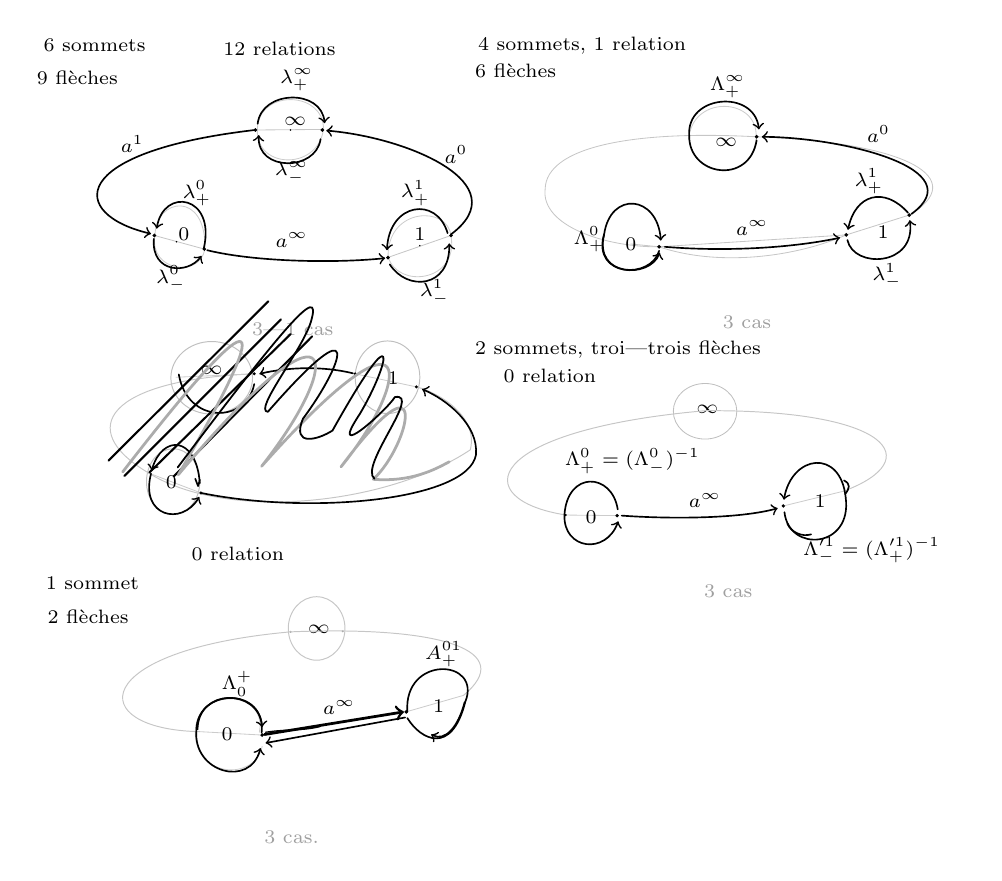
\begin{tikzpicture}[x=.0072cm,y=-.0072cm,line width=.6pt,line cap=round,line join=round,font=\scriptsize]
% Figure 1: upper left.
\node[anchor=west] at (35,42) {6 sommets};
\node[anchor=west] at (23,100) {9 flèches};
\node[anchor=west] at (352,48) {\deleted{\unsure{1}}\inserted{2} relations};
\draw[gray!45,line width=.3pt] (426,192)--(545,191);
\draw[gray!45,line width=.3pt] (248,378)--(336,402);
\draw[gray!45,line width=.3pt] (659,417)--(771,378);
\draw[gray!40,line width=.3pt] (430,185) .. controls (438,119) and (548,125) .. (546,191) .. controls (536,266) and (420,261) .. (430,185);
\draw[gray!40,line width=.3pt] (249,378) .. controls (250,311) and (340,298) .. (337,402) .. controls (328,454) and (238,441) .. (249,378);
\draw[gray!40,line width=.3pt] (660,415) .. controls (659,328) and (766,325) .. (771,379) .. controls (785,460) and (676,473) .. (660,415);
\draw[->] (430,181) .. controls (437,121) and (543,119) .. (548,180);
\draw[->] (541,208) .. controls (533,265) and (429,266) .. (432,201);
\node at (499,104) {$\lambda^\infty_+$};
\node at (490,267) {$\lambda^\infty_-$};
\node at (496,176) {$\infty$}; \fill (488,192) circle (1.4);
\draw[->] (335,401) .. controls (357,307) and (264,292) .. (252,366);
\draw[->] (247,384) .. controls (242,445) and (307,447) .. (331,414);
\node at (323,304) {$\lambda^0_+$};
\node at (277,454) {$\lambda^0_-$};
\node at (300,376) {$0$}; \fill (287,389) circle (1.5);
\draw[->] (765,374) .. controls (746,308) and (662,320) .. (658,404);
\draw[->] (663,429) .. controls (694,477) and (769,471) .. (768,392);
\node at (708,303) {$\lambda^1_+$};
\node at (742,478) {$\lambda^1_-$};
\node at (716,375) {$1$}; \fill (716,396) circle (1.4);
\draw[->] (425,192) .. controls (91,231) and (97,341) .. (242,375);
\draw[->] (771,376) .. controls (890,287) and (695,205) .. (551,193);
\draw[->] (341,404) .. controls (427,425) and (568,427) .. (655,418);
\node at (209,217) {$a^1$};
\node at (780,235) {$a^0$};
\node at (490,386) {$a^\infty$};
\foreach \x/\y in {426/192,544/192,248/378,336/402,660/417,771/378} \fill (\x,\y) circle (3.5);
% Figure 2: upper right.
\node[anchor=west] at (801,43) {4 sommets, 1 relation};
\node[anchor=west] at (796,87) {6 flèches};
\draw[gray!45,line width=.3pt] (1310,204) .. controls (1090,192) and (939,222) .. (937,296) .. controls (929,362) and (1046,399) .. (1138,398);
\draw[gray!45,line width=.3pt] (1138,398) .. controls (1241,433) and (1376,417) .. (1468,377);
\draw[gray!45,line width=.3pt] (1088,393)--(1138,398)--(1468,377)--(1579,342);
\draw[gray!45,line width=.3pt] (1579,342) .. controls (1686,279) and (1582,214) .. (1310,204);
\draw[gray!40,line width=.3pt] (1309,205) .. controls (1313,135) and (1200,130) .. (1191,203) .. controls (1194,283) and (1305,284) .. (1309,205);
\draw[->] (1310,210) .. controls (1297,290) and (1190,273) .. (1191,202) .. controls (1186,129) and (1306,120) .. (1314,191);
\node at (1259,116) {$\Lambda^\infty_+$};
\node at (1256,213) {$\infty$};
\draw[->] (1138,405) .. controls (1124,455) and (1022,453) .. (1041,376) .. controls (1052,299) and (1135,306) .. (1141,387);
\draw[->] (1041,376) .. controls (1019,451) and (1122,455) .. (1139,408);
\node at (1015,385) {$\Lambda^0_+$};
\node at (1088,394) {$0$};
\draw[->] (1148,398) .. controls (1244,406) and (1361,402) .. (1457,382);
\node at (1302,365) {$a^\infty$};
\draw[->] (1577,338) .. controls (1535,291) and (1484,305) .. (1471,368);
\draw[->] (1470,386) .. controls (1481,437) and (1591,433) .. (1580,351);
\node at (1508,283) {$\lambda^1_+$};
\node at (1540,449) {$\lambda^1_-$};
\node at (1533,372) {$1$};
\draw[->] (1583,340) .. controls (1692,261) and (1464,205) .. (1319,204);
\node at (1525,199) {$a^0$};
\foreach \x/\y in {1310/204,1138/398,1468/377,1579/342} \fill (\x,\y) circle (3.5);
\node[text=gray!75] at (1293,531) {3 cas};
% Figure 3: cancelled middle-left draft. Cancellation strokes are drawn below.
\draw[gray!50,line width=.35pt] (349,629) ellipse (72 and 64);
\draw[gray!50,line width=.35pt] (659,628) ellipse (57 and 64);
\draw[gray!50,line width=.35pt] (281,812) ellipse (47 and 58);
\draw[gray!45,line width=.35pt] (424,622) .. controls (167,632) and (105,719) .. (238,797) .. controls (374,882) and (656,855) .. (805,756) .. controls (820,695) and (746,654) .. (710,645);
\draw[gray!40,line width=.3pt] (286,628)--(424,622);
\draw[gray!40,line width=.3pt] (238,797)--(330,832);
\draw[gray!40,line width=.3pt] (602,622)--(710,645);
\node at (349,616) {$\infty$};
\node at (669,629) {$1$};
\node at (278,814) {$0$};
\node[text=gray!75] at (492,543) {\unsure{3|1} cas};
\draw[->] (598,621) .. controls (544,608) and (485,610) .. (433,622);
\draw (424,640) .. controls (410,710) and (306,711) .. (291,623);
\draw[->] (330,832) .. controls (520,871) and (800,846) .. (815,765) .. controls (820,712) and (763,667) .. (720,649);
\draw[->] (328,815) .. controls (322,730) and (261,729) .. (243,793);
\draw[->] (242,798) .. controls (222,874) and (296,891) .. (327,839);
% Pointed downward ending on the upper-right side of the cancelled 0-circle.
\draw (320,807)--(325,820)--(328,809);
\foreach \x/\y in {424/622,602/622,710/645,330/832} \fill (\x,\y) circle (2.9);
\draw[line width=.75pt] (167,775)--(449,494) (195,802)--(471,526) (239,796)--(488,552) (282,803)--(526,556);
\draw[gray!65,line width=1pt] (192,795) .. controls (450,461) and (457,515) .. (290,800) .. controls (569,467) and (591,589) .. (437,785) .. controls (716,471) and (702,633) .. (577,786) .. controls (737,571) and (700,746) .. (634,808) .. controls (701,813) and (742,791) .. (768,777);
\draw[line width=.65pt] (289,787) .. controls (471,546) and (546,455) .. (524,530) .. controls (509,580) and (422,687) .. (448,689) .. controls (618,494) and (583,603) .. (510,701) .. controls (489,752) and (537,738) .. (562,722) .. controls (685,502) and (662,606) .. (610,693) .. controls (551,782) and (657,687) .. (672,663) .. controls (721,654) and (608,785) .. (636,807);
% Figure 4: middle right.
\node[anchor=west] at (796,579) {2 sommets, \unsure{troi|trois} flèches};
\node[anchor=west] at (846,625) {0 relation};
\draw[gray!50,line width=.3pt] (1219,688) ellipse (56 and 49);
\node at (1223,684) {$\infty$};
\draw[gray!45,line width=.35pt] (974,871) .. controls (800,844) and (823,722) .. (1219,687) .. controls (1548,685) and (1611,774) .. (1463,829);
\draw[gray!40,line width=.3pt] (974,871)--(1064,872);
\draw[gray!40,line width=.3pt] (1357,855)--(1463,829);
\draw[->] (1065,861) .. controls (1055,796) and (976,792) .. (971,871) .. controls (969,932) and (1044,942) .. (1066,882);
\fill (973,871) circle (2.2); \fill (1064,872) circle (3.2);
\node at (1018,875) {$0$};
\node at (1091,775) {$\Lambda^0_+=(\Lambda^0_-)^{-1}$};
\draw[->] (1072,872) .. controls (1154,878) and (1279,878) .. (1347,859);
\node at (1219,845) {$a^\infty$};
\draw[->] (1359,866) .. controls (1367,938) and (1479,930) .. (1467,840) .. controls (1458,753) and (1372,764) .. (1358,844);
\draw (1364,886) .. controls (1371,902) and (1391,910) .. (1406,905);
\draw (1464,810) .. controls (1476,816) and (1474,824) .. (1466,834);
\fill (1357,855) circle (3.2);
\node at (1422,846) {$1$};
\node at (1513,933) {$\Lambda^{\prime1}_-=(\Lambda^{\prime1}_+)^{-1}$};
\node[text=gray!75] at (1260,1006) {3 cas};
% Figure 5: lower left.
\node[anchor=west] at (39,992) {1 sommet};
\node[anchor=west] at (42,1050) {2 flèches};
\node[anchor=west] at (296,940) {0 relation};
\draw[gray!45,line width=.35pt] (534,1071) ellipse (50 and 56);
\fill[gray!75] (488,1077) circle (2.0); \fill[gray!75] (580,1076) circle (2.0);
\node at (538,1072) {$\infty$};
\draw[gray!45,line width=.35pt] (328,1253) .. controls (123,1249) and (129,1109) .. (488,1077) .. controls (759,1066) and (887,1111) .. (793,1189);
\draw[gray!40,line width=.3pt] (328,1253)--(438,1259);
\draw[gray!40,line width=.3pt] (692,1218)--(793,1189);
\draw[gray!40,line width=.3pt] (433,1254) .. controls (448,1178) and (321,1173) .. (320,1254) .. controls (320,1335) and (426,1340) .. (438,1279);
\draw[->] (437,1255) .. controls (446,1173) and (323,1175) .. (322,1250) .. controls (315,1325) and (417,1353) .. (435,1282);
\draw[->] (324,1249) .. controls (325,1176) and (431,1176) .. (438,1245);
\node at (394,1169) {$\Lambda_0^+$};
\node at (376,1258) {$0$};
\draw[->,line width=1pt] (442,1258)--(688,1218);
\draw[line width=.45pt] (444,1254) .. controls (482,1248) and (509,1252) .. (540,1244);
\draw[->] (690,1228)--(444,1273);
\node at (574,1211) {$\deleted{\unsure{a^\infty}}$};
\draw (694,1218) .. controls (687,1117) and (827,1124) .. (796,1201) .. controls (772,1295) and (718,1268) .. (694,1229);
\draw[->] (795,1201) .. controls (784,1244) and (761,1271) .. (736,1258);
\node at (758,1117) {$A_+^{01}$};
\node at (749,1209) {$1$};
\fill (438,1259) circle (3.5); \fill (692,1218) circle (3.5);
\node[text=gray!75] at (490,1440) {3 cas.};
\end{tikzpicture}}
\mspage{105}
